\documentclass[9pt]{extarticle}
\title{}
\author{Avinash Iyer}
\date{}
\usepackage[shortlabels]{enumitem}
%font setup
%
%\usepackage[math]{anttor}

%paper setup
\usepackage{geometry}
\geometry{letterpaper, portrait, margin=1in}
\usepackage{fancyhdr}

%symbols
\usepackage{amsmath}
\usepackage{amssymb}
\usepackage{hyperref}
\usepackage{gensymb}

\usepackage[T1]{fontenc}
\usepackage[utf8]{inputenc}

%chemistry stuff
\usepackage[version=4]{mhchem}
\usepackage{chemfig}

%plotting
\usepackage{pgfplots}
\usepackage{tikz}

%\usepackage{natbib}

%graphics stuff
\usepackage{graphicx}
\graphicspath{ {./images/} }

%code stuff
%when using minted, make sure to add the -shell-escape flag
%you can use lstlisting if you don't want to use minted
%\usepackage{minted}
%\usemintedstyle{pastie}
%\newminted[javacode]{java}{frame=lines,framesep=2mm,linenos=true,fontsize=\footnotesize,tabsize=3,autogobble,}
%\newminted[cppcode]{cpp}{frame=lines,framesep=2mm,linenos=true,fontsize=\footnotesize,tabsize=3,autogobble,}

\usepackage{listings}
\usepackage{color}
\definecolor{dkgreen}{rgb}{0,0.6,0}
\definecolor{gray}{rgb}{0.5,0.5,0.5}
\definecolor{mauve}{rgb}{0.58,0,0.82}

\lstset{frame=tb,
	language=Java,
	aboveskip=3mm,
	belowskip=3mm,
	showstringspaces=false,
	columns=flexible,
	basicstyle={\small\ttfamily},
	numbers=none,
	numberstyle=\tiny\color{gray},
	keywordstyle=\color{blue},
	commentstyle=\color{dkgreen},
	stringstyle=\color{mauve},
	breaklines=true,
	breakatwhitespace=true,
	tabsize=3
}
% text + color boxes
\usepackage{tcolorbox}
\newtcolorbox{problem}[1]{colback = white, colframe = black, title = {#1}}
\newtcolorbox{solution}{colback = white, title = Solution}
%including PDFs
\usepackage{pdfpages}
\setlength{\parindent}{0pt}

\pagestyle{fancy}
\fancyhf{}
\rhead{Avinash Iyer}
\lhead{Homework Section 1.2, Individual}
\begin{document}
  \begin{problem}{1.2.1}
    Determine whether the following statements are true or false:
      \begin{itemize}
        \item Every disconnected graph has an isolated vertex.
        \item A graph is connected if and only if some vertex is connected to all other vertices.
        \item The edge set of every closed trail can be partitioned into edge sets of cycles.
        \item If a maximal trail in a graph is not closed, then its endpoints have odd degree.
      \end{itemize}
  \end{problem}
    \begin{solution}
        \begin{itemize}
          \item False
          \item True
          \item False
          \item True
        \end{itemize}
    \end{solution}
  \begin{problem}{1.2.5}
    Let $v$ be a vertex of a connected simple graph $G$. Prove that $v$ has a neighbor in every component of $G-v$. Explain why this allows us to conclude that no graph has a cut-vertex of degree 1.   
  \end{problem}
  \begin{solution}
    Suppose that $G-v$ is connected. Then, since $G$ is connected, and $v\in V(G)$, it must be the case that $v$ is connected to every component of $G-v$, meaning that it has a neighbor in every component of $G-v$ as $G-v$ is connected.\\

    Now suppose that $G-v$ is disconnected, meaning that it has more than one component after removing $v$. Before, $v$ must have been connected to every vertex in $G$ as $G$ was a simple connected graph, and afterwards $G-v$ is no longer connected, meaning that $v$ is a cut-vertex. This means $v$ must have been adjacent to a vertex in each component of $G-v$, as removing the incident edges on $v$ along with $v$ increased the number of components from the original $1$ that was in $G$.\\

    From this result, we can conclude that no cut-vertex has degree $1$ as removing a vertex of degree $1$ and its incident edges does not increase the number of components in $G$, since there is only one edge incident on a vertex of degree $1$.
  \end{solution}
  \begin{problem}{1.2.6}
    In the graph below, find all the maximal paths, maximal cliques, and maximal independent sets. Also, find all the maximum paths, cliques, and independent sets. 
      \begin{center}
          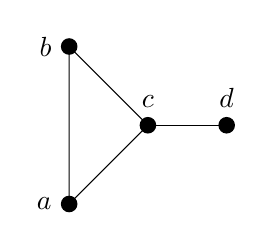
\begin{tikzpicture}
            \fill (0,0) circle (3pt);
            \fill (-1,1) circle (3pt);
            \fill (-1,-1) circle (3pt);
            \fill (1,0) circle (3pt);
            \node[anchor = south] at (0,0.1) {$c$};
            \node[anchor = south] at (1,0.1) {$d$};
            \node[anchor = east] at (-1.1,-1) {$a$};
            \node[anchor = east] at (-1.1,1) {$b$};
            \draw (-1,-1) -- (-1,1) -- (0,0) -- (-1,-1);
            \draw (0,0) -- (1,0);
          \end{tikzpicture}
      \end{center}
  \end{problem}
  \begin{solution}
    \begin{itemize}
        \item The maximal paths are as follows:
       \begin{itemize}
         \item $d,c,b,a$
         \item $d,c,a,b$
         \item $a,b,c,d$
         \item $b,a,c,d$
         \item $b,c,a$
         \item $c,b,a$
         \item $a,c,b$
       \end{itemize}
     \item The maximal cliques are $K_3$ consisting of $a,b,c$ and $K_2$ consisting of $c,d$.
     \item The maximal independent sets are $\{a,d\}$ and  $\{b,d\}$.
     \item The maximum path is any of those paths listed above with length $4$.
     \item The maximum clique is $K_3$.
     \item The maximum independent sets are those listed above with size $2$.
    \end{itemize}
  \end{solution}
  \begin{problem}{1.2.8}
    Determine the values of $m$ and $n$ such that $K_{m,n}$ is Eulerian. 
  \end{problem}
  \begin{solution}
    \[
      m,n\in 2\mathbb{Z}^{+}
    \]
  \end{solution}
  \begin{problem}{1.2.10}
      Prove or disprove:
      \begin{enumerate}[(a)]
          \item Every Eulerian bipartite graph has an even number of edges.
          \item Every Eulerian simple graph with an even number of vertices has an even number of edges.
        \end{enumerate}
  \end{problem}
    \begin{solution}
      \begin{tcolorbox}[colback = white, title = (a)]
        Let $G$ be an Eulerian bipartite graph. Since $G$ is Eulerian, it must contain an Eulerian cycle, meaning that as seen above, there are an even number of vertices, meaning that there are an even number of edges in $G$. 
      \end{tcolorbox}

      \begin{tcolorbox}[colback = white, title = (b)]
        Let $G$ be an Eulerian simple graph with an even number of vertices. Since $G$ is Eulerian, this means there must be an Eulerian circuit $C$ that traverses every edge exactly once in $G$. Every vertex in $G$ must have even degree (or else we would require a backtrack in our Eulerian cycle, which is not a circuit); a simple pairing of the vertices would yield that we have $\lfloor n/2\rfloor $ edges, and to complete the cycle we need $2(n/2) + 2k$ edges for $n$ vertices and some integer $k$. Therefore, there must be an even number of edges.
      \end{tcolorbox}
    \end{solution}
\end{document}
